\documentclass[12pt, a4paper]{report}
\usepackage{epsfig}
\usepackage{subfigure}
%\usepackage{amscd}
\usepackage{amssymb}
\usepackage{graphicx}
%\usepackage{amscd}
\usepackage{amssymb}
\usepackage{amsthm, amsmath}
\usepackage{amsbsy}
\usepackage[usenames]{color}
\usepackage{listings}
\lstset{% general command to set parameter(s)
basicstyle=\small, % print whole listing small
keywordstyle=\color{red}\itshape,
% underlined bold black keywords
commentstyle=\color{blue}, % white comments
stringstyle=\ttfamily, % typewriter type for strings
showstringspaces=false,
numbers=left, numberstyle=\tiny, stepnumber=1, numbersep=5pt, %
frame=shadowbox,
rulesepcolor=\color{black},
,columns=fullflexible
} %
%\usepackage[dvips]{graphicx}
\usepackage{natbib}
\bibliographystyle{chicago}
\usepackage{vmargin}
% left top textwidth textheight headheight
% headsep footheight footskip
\setmargins{3.0cm}{2.5cm}{15.5 cm}{22cm}{0.5cm}{0cm}{1cm}{1cm}
\renewcommand{\baselinestretch}{1.5}
\pagenumbering{arabic}
\theoremstyle{plain}
\newtheorem{theorem}{Theorem}[section]
\newtheorem{corollary}[theorem]{Corollary}
\newtheorem{ill}[theorem]{Example}
\newtheorem{lemma}[theorem]{Lemma}
\newtheorem{proposition}[theorem]{Proposition}
\newtheorem{conjecture}[theorem]{Conjecture}
\newtheorem{axiom}{Axiom}
\theoremstyle{definition}
\newtheorem{definition}{Definition}[section]
\newtheorem{notation}{Notation}
\theoremstyle{remark}
\newtheorem{remark}{Remark}[section]
\newtheorem{example}{Example}[section]
\renewcommand{\thenotation}{}
\renewcommand{\thetable}{\thesection.\arabic{table}}
\renewcommand{\thefigure}{\thesection.\arabic{figure}}
\title{Research notes: linear mixed effects models}
\author{ } \date{ }


\begin{document}
\author{Kevin O'Brien}
\title{Mixed Models for Method Comparison Studies}

%----------------------------------------------------------------------------------------%
\newpage
\chapter{Method Comparison Studies}

\section{Introduction}
The problem of assessing the agreement between two or more methods
of measurement is ubiquitous in scientific research, and is
commonly referred to as a `method comparison study'. Published
examples of method comparison studies can be found in disciplines
as diverse as pharmacology \citep{ludbrook97}, anaesthesia
\citep{Myles}, and cardiac imaging methods \citep{Krumm}.
\smallskip

To illustrate the characteristics of a typical method comparison
study consider the data in Table I \citep{Grubbs73}. In each of
twelve experimental trials, a single round of ammunition was fired
from a 155mm gun and its velocity was measured simultaneously (and
independently) by three chronographs devices, identified here by
the labels `Fotobalk', `Counter' and `Terma'.
\smallskip


\newpage

\begin{table}[ht]
\begin{center}
\begin{tabular}{rrrr}
  \hline
  Round& Fotobalk [F] & Counter [C]& Terma [T]\\
  \hline
  1 & 793.8 & 794.6 & 793.2 \\
  2 & 793.1 & 793.9 & 793.3 \\
  3 & 792.4 & 793.2 & 792.6 \\
  4 & 794.0 & 794.0 & 793.8 \\
  5 & 791.4 & 792.2 & 791.6 \\
  6 & 792.4 & 793.1 & 791.6 \\
  7 & 791.7 & 792.4 & 791.6 \\
  8 & 792.3 & 792.8 & 792.4 \\
  9 & 789.6 & 790.2 & 788.5 \\
  10 & 794.4 & 795.0 & 794.7 \\
  11 & 790.9 & 791.6 & 791.3 \\
  12 & 793.5 & 793.8 & 793.5 \\
   \hline
\end{tabular}
\caption{Velocity measurement from the three chronographs (Grubbs
1973).}
\end{center}
\end{table}

An important aspect of the these data is that all three methods of
measurement are assumed to have an attended measurement error, and
the velocities reported in Table 1.1 can not be assumed to be
`true values' in any absolute sense.

%While lack of
%agreement between two methods is inevitable, the question , as
%posed by \citet{BA83}, is 'do the two methods of measurement agree
%sufficiently closely?'

A method of measurement should ideally be both accurate and
precise. \citet{Barnhart} describes agreement as being a broader
term that contains both of those qualities. An accurate
measurement method will give results close to the unknown `true
value'. The precision of a method is indicated by how tightly
measurements obtained under identical conditions are distributed
around their mean measurement value. A precise and accurate method
will yield results consistently close to the true value. Of course
a method may be accurate, but not precise, if the average of its
measurements is close to the true value, but those measurements
are highly dispersed. Conversely a method that is not accurate may
be quite precise, as it consistently indicates the same level of
inaccuracy. The tendency of a method of measurement to
consistently give results above or below the true value is a
source of systematic bias. The smaller the systematic bias, the
greater the accuracy of the method.

% The FDA define precision as the closeness of agreement (degree of
% scatter) between a series of measurements obtained from multiple
% sampling of the same homogeneous sample under prescribed
% conditions. \citet{Barnhart} describes precision as being further
% subdivided as either within-run, intra-batch precision or
% repeatability (which assesses precision during a single analytical
% run), or between-run, inter-batch precision or repeatability
%(which measures precision over time).

In the context of the agreement of two methods, there is also a
tendency of one measurement method to consistently give results
above or below the other method. Lack of agreement is a
consequence of the existence of `inter-method bias'. For two
methods to be considered in good agreement, the inter-method bias
should be in the region of zero. A simple estimation of the
inter-method bias can be calculated using the differences of the
paired measurements. The data in Table 1.2 are a good example of
possible inter-method bias; the `Fotobalk' consistently recording
smaller velocities than the `Counter' method. Consequently one
would conclude that there is lack of agreement between the two
methods.

The absence of inter-method bias by itself is not sufficient to
establish whether two measurement methods agree. The two methods
must also have equivalent levels of precision. Should one method
yield results considerably more variable than those of the other,
they can not be considered to be in agreement. With this in mind a
methodology is required that allows an analyst to estimate the
inter-method bias, and to compare the precision of both methods of
measurement.
\newpage
% latex table generated in R 2.6.0 by xtable 1.5-5 package
% Wed Aug 26 15:22:41 2009
\begin{table}[h!]

\begin{center}

\begin{tabular}{rrrr}
  \hline
 Round& Fotobalk (F) & Counter (C) & F-C \\
  \hline
1 & 793.8& 794.6 & -0.8 \\
  2 & 793.1 & 793.9 & -0.8 \\
  3 & 792.4 & 793.2 & -0.8 \\
  4 & 794.0 & 794.0 & 0.0 \\
  5 & 791.4 & 792.2 & -0.8 \\
  6 & 792.4 & 793.1 & -0.7 \\
  7 & 791.7 & 792.4 & -0.7 \\
  8 & 792.3 & 792.8 & -0.5 \\
  9 & 789.6 & 790.2 & -0.6 \\
  10 & 794.4 & 795.0 & -0.6 \\
  11 & 790.9 & 791.6 & -0.7 \\
  12 & 793.5 & 793.8 & -0.3 \\
   \hline
\end{tabular}
\caption{Difference between Fotobalk and Counter measurements.}
\end{center}
\end{table}

\bigskip

\newpage

\section{Bland-Altman methodology}
The issue of whether two measurement methods comparable to the
extent that they can be used interchangeably with sufficient
accuracy is encountered frequently in scientific research.
Historically comparison of two methods of measurement was carried
out by use of paired sample $t-$test, correlation coefficients or
simple linear regression. Simple linear regression is unsuitable for method comparison studies because of the required assumption that one variable is measured without error. In comparing two methods, both methods are assume to have attendant random error.

Statisticians Martin Bland and Douglas Altman recognized the inadequacies of these analyzes and
articulated quite thoroughly the basis on which of which they are unsuitable for comparing two methods of measurement \citep*{BA83}. Furthermore they proposed their simple methodology specifically
constructed for method comparison studies. They acknowledge the opportunity to apply other valid, but complex, methodologies, but argue that a simple approach is preferable, especially when the
results must be `explained to non-statisticians'.

Notwithstanding previous remarks about linear regression, the first step recommended, which the authors argue should be mandatory, is construction of a simple scatter plot of the data. The line of equality should also be shown, as it is necessary to give the correct interpretation of how both methods compare. In the case of good agreement, the observations would be distributed closely along the line of equality. A scatter plot of the Grubbs data is shown in Figure 1.1. Visual inspection confirms the previous conclusion that there is an inter-method bias present, i.e. Fotobalk device has a tendency to record a lower velocity.

\begin{figure}[h!]
\begin{center}
  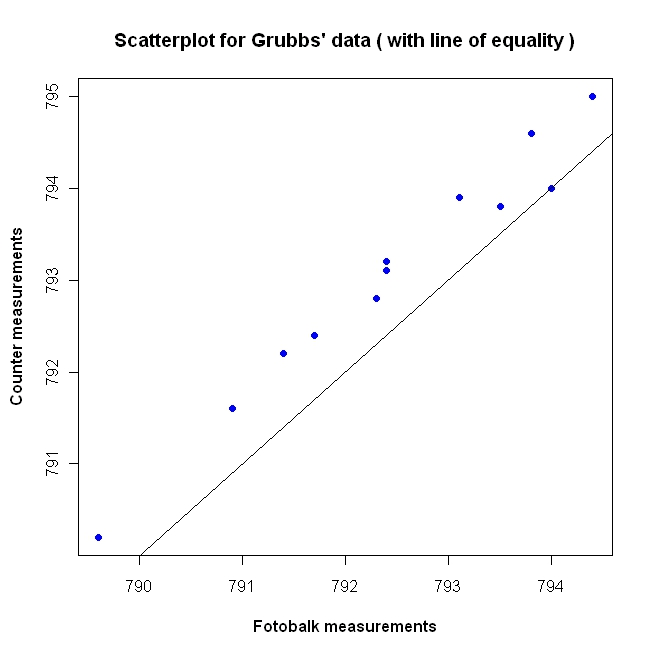
\includegraphics[width=125mm]{GrubbsScatter.jpeg}
  \caption{Scatter plot For Fotobalk and Counter Methods.}\label{GrubbsScatter}
\end{center}
\end{figure}

\citet{Dewitte} notes that scatter plots were very seldom
presented in the Annals of Clinical Biochemistry. This apparently
results from the fact that the `Instructions for Authors' dissuade
the use of regression analysis, which conventionally is
accompanied by a scatter plot.

\newpage
\subsection{Bland-Altman plots}

In light of shortcomings associated with scatterplots,
\citet*{BA83} recommend a further analysis of the data. Firstly
case-wise differences of measurements of two methods $d_{i} =
y_{1i}-y_{2i} \mbox{ for }i=1,2,\dots,n$ on the same subject
should be calculated, and then the average of those measurements
($a_{i} = (y_{1i} + y_{2i})/2 \mbox{ for }i=1,2,\dots, n$).

\citet{BA83} proposes a scatterplot of the case-wise averages and differences of two methods of measurement. This scatterplot has since become widely known as the Bland-Altman plot. \citet*{BA83} express the
motivation for this plot thusly:
\begin{quote}
``From this type of plot it is much easier to assess the magnitude
of disagreement (both error and bias), spot outliers, and see
whether there is any trend, for example an increase in (difference) for high values. This way of plotting the data is a very powerful way of displaying the results of a method comparison study."
\end{quote}

The case wise-averages capture several aspects of the data, such as expressing the range over which the values were taken, and assessing whether the assumptions of constant variance holds.
Case-wise averages also allow the case-wise differences to be presented on a two-dimensional plot, with better data visualization qualities than a one dimensional plot. \citet{BA86}
cautions that it would be the difference against either measurement value instead of their average, as the difference relates to both value. This methodology has proved very popular, and the Bland-Altman plots is widely regarded as powerful graphical methodology for making a visual assessment of the data.

The magnitude of the inter-method bias between the two methods is simply the average of the differences $\bar{d}$. This inter-method bias is represented with a line on the Bland-Altman plot. As the objective of the Bland-Altman plot is to advise on the agreement of two methods, it is the case-wise differences that are also particularly relevant. The variances around this bias is estimated by the standard deviation of these differences $S_{d}$.

\subsection{Bland-Altman plots for the Grubbs data}

In the case of the Grubbs data the inter-method bias is $-0.61$ metres per second, and is indicated by the dashed line on Figure 1.2. By inspection of the plot, it is also possible to compare the precision of each method. Noticeably the differences tend to increase as the averages increase.


The Bland-Altman plot for comparing the `Fotobalk' and `Counter'
methods, which shall henceforth be referred to as the `F vs C'
comparison,  is depicted in Figure 1.2, using data from Table 1.3.
The presence and magnitude of the inter-method bias is indicated
by the dashed line.
\newpage

%Later it will be shown that case-wise differences are the sole
%component of the next part of the methodology, the limits of
%agreement.


\begin{table}[h!]
\renewcommand\arraystretch{0.7}%
\begin{center}
\begin{tabular}{|c||c|c||c|c|}
  \hline
 Round & Fotobalk  & Counter  & Differences  & Averages  \\
  &  [F] & [C] & [F-C] &  [(F+C)/2] \\
  \hline
1 & 793.8 & 794.6 & -0.8 & 794.2 \\
  2 & 793.1 & 793.9 & -0.8 & 793.5 \\
  3 & 792.4 & 793.2 & -0.8 & 792.8 \\
  4 & 794.0 & 794.0 & 0.0 & 794.0 \\
  5 & 791.4 & 792.2 & -0.8 & 791.8 \\
  6 & 792.4 & 793.1 & -0.7 & 792.8 \\
  7 & 791.7 & 792.4 & -0.7 & 792.0 \\
  8 & 792.3 & 792.8 & -0.5 & 792.5 \\
  9 & 789.6 & 790.2 & -0.6 & 789.9 \\
  10 & 794.4 & 795.0 & -0.6 & 794.7 \\
  11 & 790.9 & 791.6 & -0.7 & 791.2 \\
  12 & 793.5 & 793.8 & -0.3 & 793.6 \\
   \hline
\end{tabular}
\caption{Fotobalk and Counter methods: differences and averages.}
\end{center}
\end{table}

\begin{table}[h!]
\renewcommand\arraystretch{0.7}%
\begin{center}
\begin{tabular}{|c||c|c||c|c|}
  \hline
 Round & Fotobalk  & Terma  & Differences  & Averages  \\
  &  [F] & [T] & [F-T] &  [(F+T)/2] \\
  \hline
1 & 793.8 & 793.2 & 0.6 & 793.5 \\
  2 & 793.1 & 793.3 & -0.2 & 793.2 \\
  3 & 792.4 & 792.6 & -0.2 & 792.5 \\
  4 & 794.0 & 793.8 & 0.2 & 793.9 \\
  5 & 791.4 & 791.6 & -0.2 & 791.5 \\
  6 & 792.4& 791.6 & 0.8 & 792.0 \\
  7 & 791.7 & 791.6 & 0.1 & 791.6 \\
  8 & 792.3 & 792.4 & -0.1 & 792.3 \\
  9 & 789.6 & 788.5 & 1.1 & 789.0 \\
  10 & 794.4 & 794.7 & -0.3 & 794.5 \\
  11 & 790.9 & 791.3 & -0.4 & 791.1 \\
  12 & 793.5 & 793.5 & 0.0 & 793.5 \\

   \hline
\end{tabular}
\caption{Fotobalk and Terma methods: differences and averages.}
\end{center}
\end{table}

\newpage

\begin{figure}[h!]
\begin{center}
  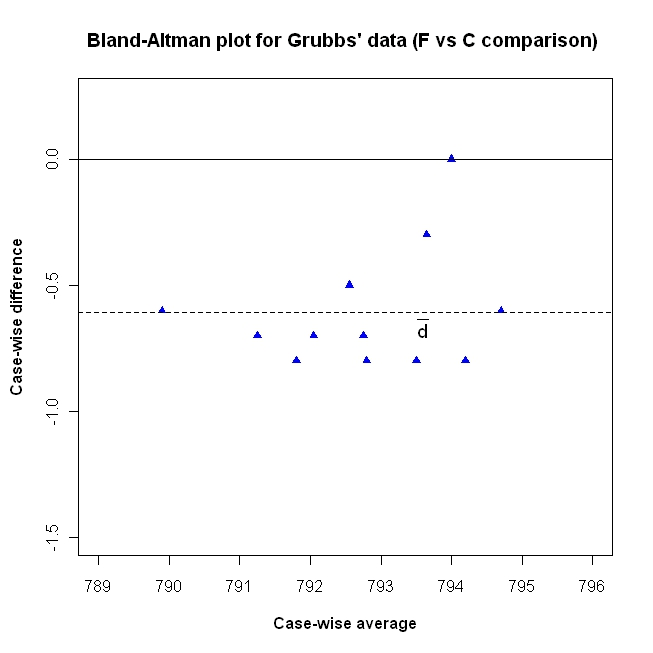
\includegraphics[width=120mm]{GrubbsBAplot-noLOA.jpeg}
  \caption{Bland-Altman plot For Fotobalk and Counter methods.}\label{GrubbsBA-noLOA}
\end{center}
\end{figure}



In Figure 1.3 Bland-Altman plots for the `F vs C' and `F vs T'
comparisons are shown, where `F vs T' refers to the comparison of
the `Fotobalk' and `Terma' methods. Usage of the Bland-Altman plot
can be demonstrate in the contrast between these comparisons. By inspection, there exists a larger inter-method bias in the `F vs C' comparison than in the `F vs T' comparison. Conversely there
appears to be less precision in `F vs T' comparison, as indicated
by the greater dispersion of covariates.

\begin{figure}[h!]
\begin{center}
  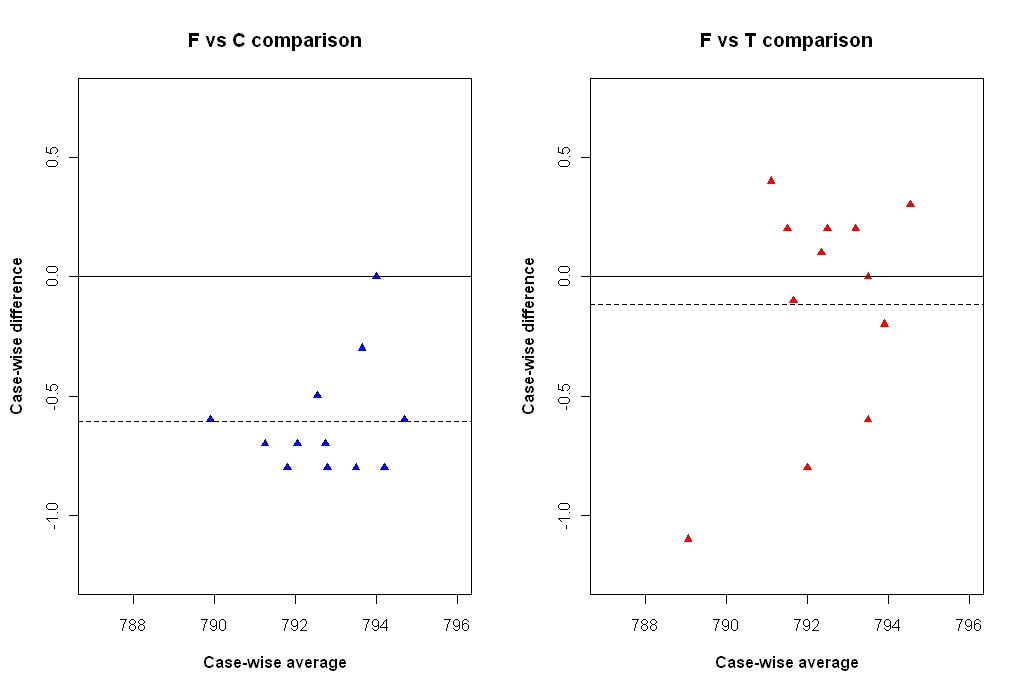
\includegraphics[height=90mm]{GrubbsDataTwoBAplots.jpeg}
  \caption{Bland-Altman plots for Grubbs' F vs C and F vs T comparisons.}\label{GrubbsDataTwoBAplots}
\end{center}
\end{figure}

\newpage


\subsection{Adverse features}

Estimates for inter-method bias and variance of differences are only meaningful if there is uniform inter-bias and variability throughout the range of measurements. Fulfilment of these assumptions can be checked by visual inspection of the plot.The prototype Bland-Altman plots depicted in Figures 1.4, 1.5 and 1.6 are derived from simulated data, for the purpose of demonstrating how the plot would inform an analyst of features that would adversely affect use of the recommended methodology.

Figure 1.4 demonstrates how the Bland-Altman plot would indicate
increasing variance of differences over the measurement range.
Fitted regression lines, for both the upper and lower half of the
plot, has been added to indicate the trend. Figure 1.5 is an
example of cases where the inter-method bias changes over the
measurement range. This is known as proportional bias, and is
defined by \citet{ludbrook97} as meaning that `one method gives
values that are higher (or lower) than those from the other by an
amount that is proportional to the level of the measured
variable'. In both Figures 1.4 and 1.5, the assumptions necessary
for further analysis using the limits of agreement are violated.

Application of regression techniques to the Bland-Altman plot, and
subsequent formal testing for the constant variability of
differences is informative. The data set may be divided into two
subsets, containing the observations wherein the difference values
are less than and greater than the inter-method bias respectively.
For both of these fits, hypothesis tests for the respective slopes
can be performed. While both tests can be considered separately,
multiple comparison procedures, such as the Benjamini-Hochberg
\citep{BH} test, should be also be used.

\begin{figure}[h!]
\begin{center}
  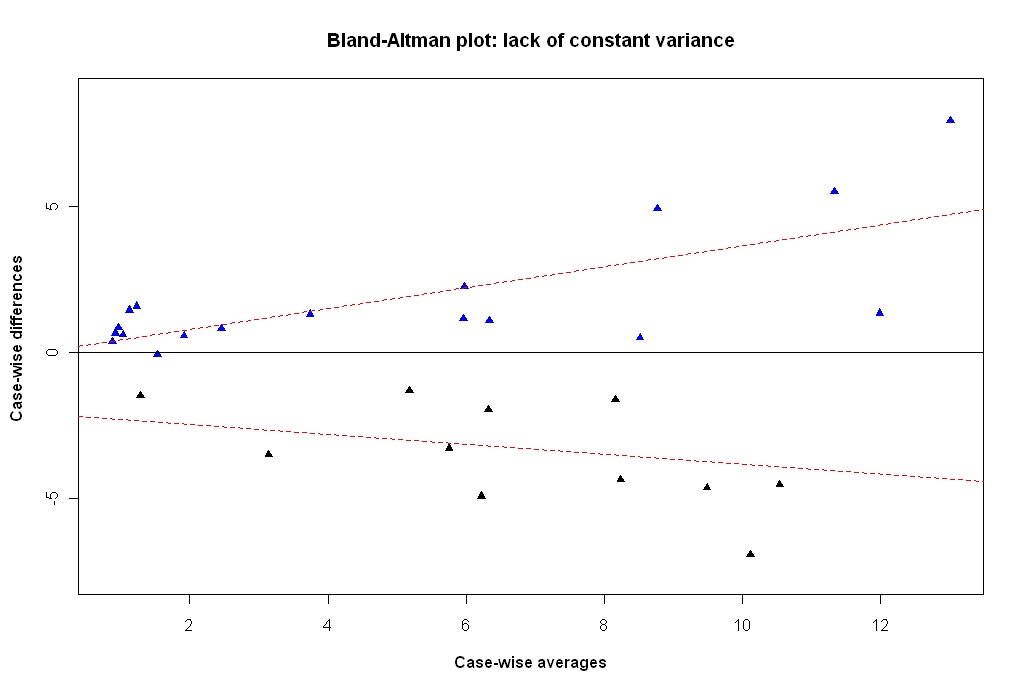
\includegraphics[height=90mm]{BAFanEffect.jpeg}
  \caption{Bland-Altman plot demonstrating the increase of variance over the range.}\label{BAFanEffect}
\end{center}
\end{figure}

\begin{figure}[h!]
\begin{center}
  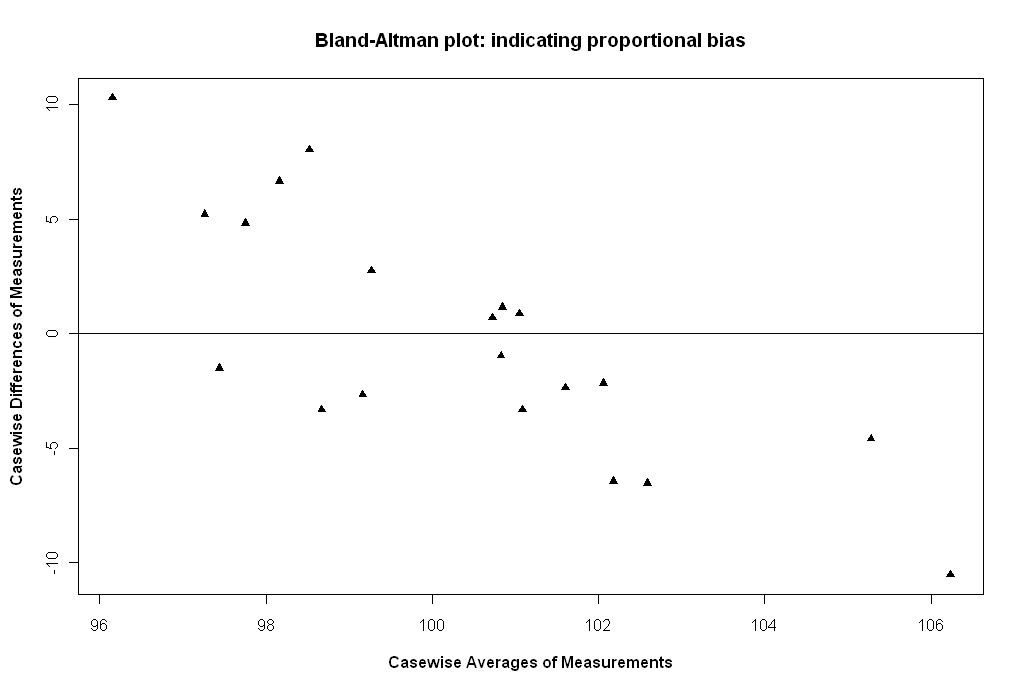
\includegraphics[height=90mm]{PropBias.jpeg}
  \caption{Bland-Altman plot indicating the presence of proportional bias.}\label{PropBias}
\end{center}
\end{figure}

\begin{figure}[h!]
\begin{center}
  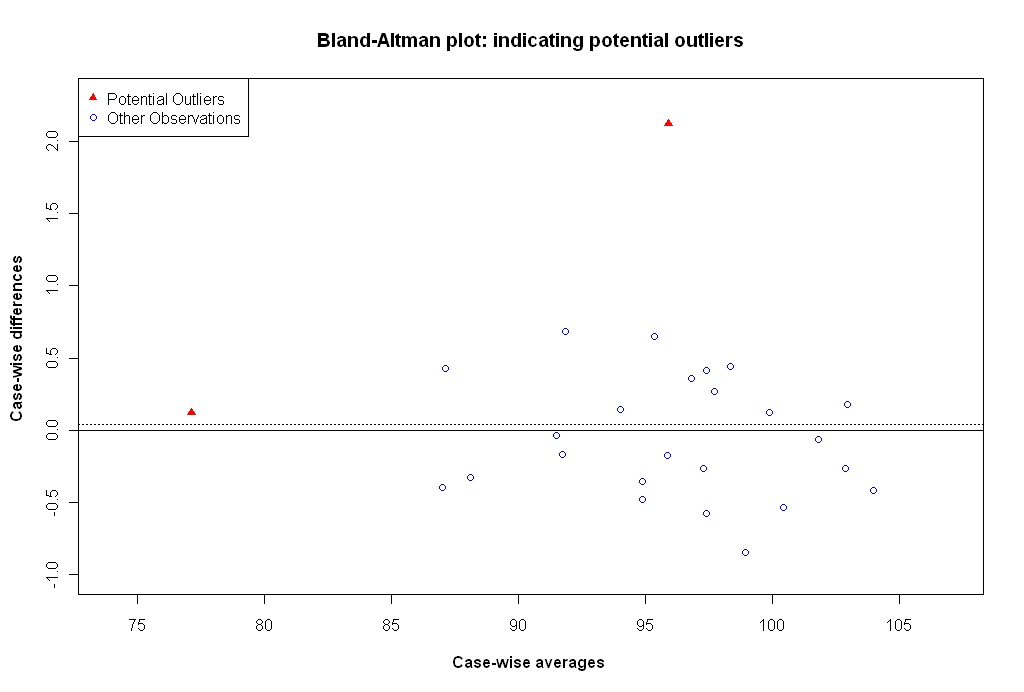
\includegraphics[width=125mm]{BAOutliers.jpeg}
  \caption{Bland-Altman plot indicating the presence of potential outliers.}\label{Outliers}
\end{center}
\end{figure}

\newpage


The Bland-Altman plot also can be used to identify outliers. An
outlier is an observation that is conspicuously different from the
rest of the data that it arouses suspicion that it occurs due to a
mechanism, or conditions, different to that of the rest of the
observations. \citet*{BA99} do not recommend excluding outliers from analyzes,
but remark that recalculation of the inter-method bias estimate,
and further calculations based upon that estimate, are useful for
assessing the influence of outliers. The authors remark that `we
usually find that this method of analysis is not too sensitive to
one or two large outlying differences'. Figure 1.6 demonstrates how the Bland-Altman
plot can be used to visually inspect the presence of potential
outliers.

As a complement to the Bland-Altman plot, \citet{Bartko} proposes
the use of a bivariate confidence ellipse, constructed for a
predetermined level. \citet{AltmanEllipse} provides the relevant calculations for the
ellipse. This ellipse is intended as a visual
guidelines for the scatter plot, for detecting outliers and to
assess the within- and between-subject variances.

The minor axis relates to the between subject variability, whereas
the major axis relates to the error mean square, with the ellipse
depicting the size of both relative to each other.
Consequently Bartko's ellipse provides a visual aid to determining the
relationship between variances. If $\mbox{var}(a)$ is greater than $\mbox{var}(d)$, the orientation of the ellipse is horizontal. Conversely if $\mbox{var}(a)$ is less than $\mbox{var}(d)$, the orientation of the ellipse is vertical.


%(Furthermore \citet{Bartko}
%proposes formal testing procedures, that shall be discussed in due
%course.)

The Bland-Altman plot for the Grubbs data, complemented by Bartko's ellipse, is depicted in Figure 1.7.
The fourth observation is shown to be outside the bounds of the ellipse, indicating that it is a potential outlier.


\begin{figure}[h!]
  % Requires \usepackage{graphicx}
  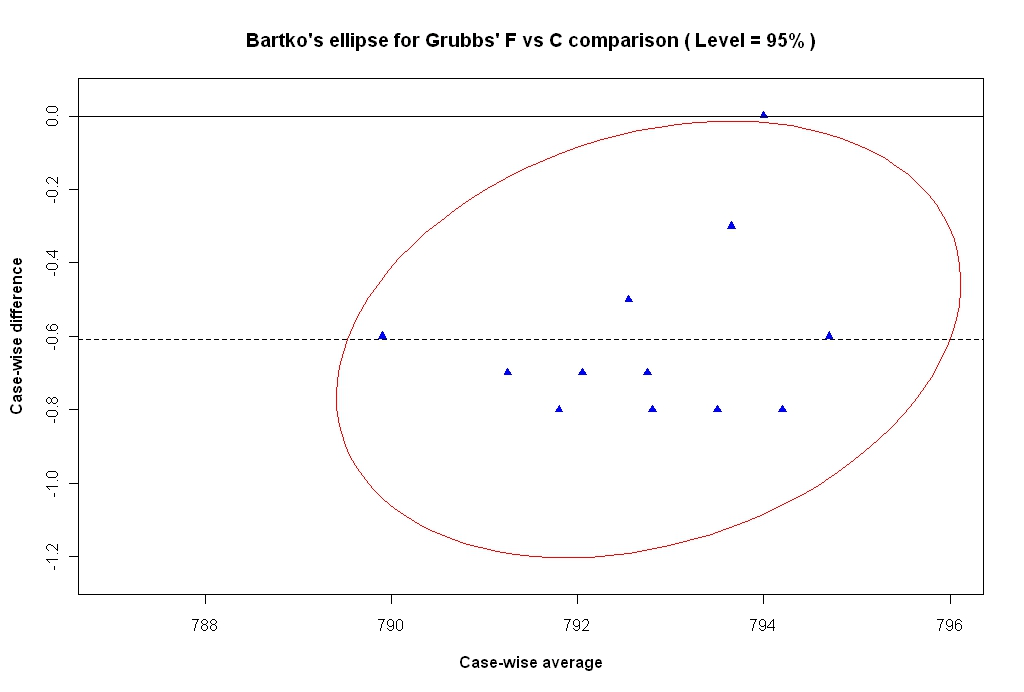
\includegraphics[width=130mm]{GrubbsBartko.jpeg}
  \caption{Bartko's Ellipse For Grubbs' Data.}\label{GrubbsBartko}
\end{figure}

The limitations of using bivariate approaches to outlier detection
in the Bland-Altman plot can demonstrated using Bartko's ellipse.
A covariate is added to the `F vs C' comparison that has a
difference value equal to the inter-method bias, and an average
value that markedly deviates from the rest of the average values
in the comparison, i.e. 786. Table 1.8 depicts a $95\%$ confidence
ellipse for this manipulated data set. By inspection of the
confidence interval, a conclusion would be reached that this extra
covariate is an outlier, in spite of the fact that this
observation is wholly consistent with the conclusion of the
Bland-Altman plot.

\begin{figure}[h!]
  % Requires \usepackage{graphicx}
  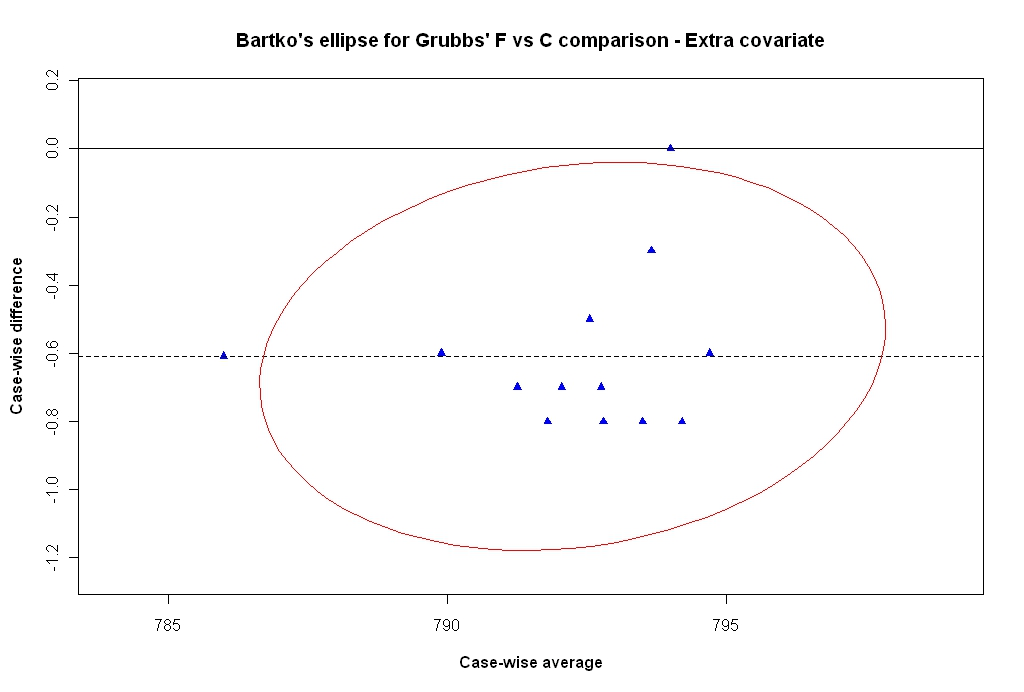
\includegraphics[width=130mm]{GrubbsBartko2.jpeg}
  \caption{Bartko's Ellipse For Grubbs' Data, with an extra covariate.}\label{GrubbsBartko2}
\end{figure}


Importantly, outlier classification must be informed by the logic of the
data's formulation. In the Bland-Altman plot, the horizontal displacement of any
observation is supported by two independent measurements. Any
observation should not be considered an outlier on the basis of a
noticeable horizontal displacement from the main cluster, as in
the case with the extra covariate. Conversely, the fourth
observation, from the original data set, should be considered an
outlier, as it has a noticeable vertical displacement from the
rest of the observations.

%Grubbs' test is a statistical test used for detecting outliers in a
%univariate data set that is assumed to be normally distributed.

%\citet{Grubbs} defined an outlier as a co-variate that appears to
%deviate markedly from other members of the sample in which it
%occurs.

In classifying whether a observation from a univariate data set is
an outlier, many formal tests are available, such as the Grubbs test for outliers. In assessing
whether a covariate in a Bland-Altman plot is an outlier, this
test is useful when applied to the case-wise difference values treated as a
univariate data set. The null hypothesis of the Grubbs test procedure is the absence
of any outliers in the data set. Conversely, the alternative hypotheses is that there is at least one outlier
present.

The test statistic for the Grubbs test ($G$) is the largest
absolute deviation from the sample mean divided by the standard
deviation of the differences,
\[
G =  \displaystyle\max_{i=1,\ldots, n}\frac{\left \vert d_i -
\bar{d}\right\vert}{S_{d}}.
\]

For the `F vs C' comparison it is the fourth observation gives
rise to the test statistic, $G = 3.64$. The critical value is
calculated using Student's $t$ distribution and the sample size,
\[
U = \frac{n-1}{\sqrt{n}} \sqrt{\frac{t_{\alpha/(2n),n-2}^2}{n - 2
+ t_{\alpha/(2n),n-2}^2}}.
\]
For this test $U = 0.75$. The conclusion of this test is that the fourth observation in the `F vs C' comparison is an outlier, with $p-$value = 0.003, according with the previous result using Bartko's ellipse.

\newpage


\section{Limits of Agreement}
% introduces
A third element of the Bland-Altman methodology, an interval known
as `limits of agreement' is introduced in \citet*{BA86}
(sometimes referred to in literature as 95\% limits of agreement).
Limits of agreement are used to assess whether the two methods of
measurement can be used interchangeably. \citet{BA86} refer to
this as the `equivalence' of two measurement methods. The specific purpose of the limits of
agreement must be
established clearly. \citet*{BA95} comment that the limits of agreement `how
far apart measurements by the two methods were likely to be for
most individuals', a definition echoed in their 1999 paper:

\begin{quote}"We can then say that nearly all pairs
of measurements by the two methods will be closer together than
these extreme values, which we call 95\% limits of agreement.
These values define the range within which most differences
between measurements by the two methods will lie."
\end{quote}

The limits of agreement (LoA) are computed by the following
formula:
\[
LoA = \bar{d} \pm 1.96 s_{d}
\]
with $\bar{d}$ as the estimate of the inter method bias, $s_{d}$
as the standard deviation of the differences and 1.96 is the 95\%
quantile for the standard normal distribution. (Some accounts of
Bland-Altman plots use a multiple of 2 standard deviations instead
for simplicity.)

The limits of agreement methodology assumes a constant level of bias throughout the range of measurements. Importantly the authors recommend prior determination of what would and would constitute acceptable
agreement, and that sample sizes should be predetermined to give an accurate conclusion. However \citet{mantha} highlights inadequacies in the correct application of limits of agreement, resulting in contradictory estimates limits of agreement in various papers.

\begin{quote}
``How far apart measurements can be without causing difficulties
will be a question of judgment. Ideally, it should be defined in
advance to help in the interpretation of the method comparison and
to choose the sample size \citep{BA86}".
\end{quote}


For the Grubbs `F vs C' comparison, these limits
of agreement are calculated as -0.132 for the upper bound, and
-1.08 for the lower bound. Figure 1.9 shows the resultant
Bland-Altman plot, with the limits of agreement shown in dashed
lines.


\begin{figure}[h!]
\begin{center}
  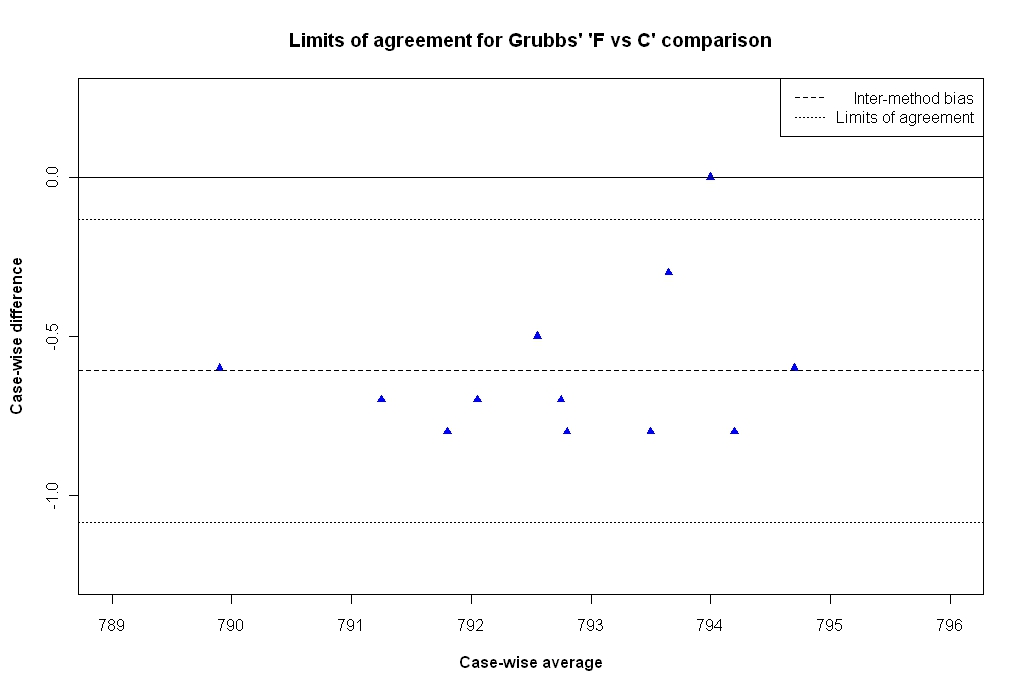
\includegraphics[width=125mm]{GrubbsBAplot-LOA.jpeg}
  \caption{Bland-Altman plot with limits of agreement}\label{GrubbsBAplot-noLOA}
\end{center}
\end{figure}

%But as \citet*{BA86} point out this may not be the case. Variants of the limits of agreement that overcome this
% problem shall be introduced in due course.

\subsection{Inferences on Bland-Altman estimates}
\citet*{BA99}advises on how to calculate confidence intervals for the inter-method bias and limits of agreement.
For the inter-method bias, the confidence interval is a simply that of a mean: $\bar{d} \pm t_{(0.5\alpha,n-1)} S_{d}/\sqrt{n}$.
The confidence
intervals and standard error for the limits of agreement follow from the variance of the limits of agreement, which is shown to be

 \[
  \mbox{Var}(LoA) = (\frac{1}{n}+\frac{1.96^{2}}{2(n-1)})s_{d}^{2}.
 \]

If $n$ is sufficiently large this can be following approximation
can be used
 \[
  \mbox{Var}(LoA) \approx 1.71^{2}\frac{s_{d}^{2}}{n}.
 \]
Consequently the standard errors of both limits can be
approximated as $1.71$ times the standard error of the
differences.

A $95\%$ confidence interval can be determined, by means of the
\emph{t} distribution with $n-1$ degrees of freedom. However \citet*{BA99} comment that such calculations  may be `somewhat optimistic' on account of the associated assumptions not being realized.

%\subsubsection{Small Sample Sizes} The limits of agreement are
%estimates derived from the sample studied, and will differ from
%values relevant to the whole population, hence the importance of a
%suitably large sample size. A different sample would give
%different limits of agreement. Student's t-distribution is a well
%known probability distribution used in statistical inference for
%normally distributed populations when the sample size is small
%\citep{student,Fisher3}. Consequently, using 't' quantiles , as
%opposed to standard normal quantiles, may give a more appropriate
%calculation for limits of agreement when the sample size is small.
%For sample size $n=12$ the `t' quantile is 2.2 and the limits of
%agreement are (-0.074,-1.143).


\subsection{Formal definition of limits of agreement}
\citet{BA99} note the similarity of limits of agreement to
confidence intervals, but are clear that they are not the same
thing. Interestingly, they describe the limits as `being like a
reference interval'.

Limits of agreement have very similar construction to Shewhart
control limits. The Shewhart chart is a well known graphical
methodology used in statistical process control. Consequently
there is potential for misinterpreting the limits of agreement as
if equivalent to Shewhart control limits. Importantly the
parameters used to determine the Shewhart limits are not based on any sample used for an analysis, but
on the process's historical values, a key difference with
Bland-Altman limits of agreement.

\citet{BXC2008} regards the limits of agreement as a prediction
interval for the difference between future measurements with the
two methods on a new individual, but states that it does not fit
the formal definition of a prediction interval, since the
definition does not consider the errors in estimation of the
parameters. Prediction intervals, which are often used in
regression analysis, are estimates of an interval in which future
observations will fall, with a certain probability, given what has
already been observed. \citet{BXC2008} offers an alternative
formulation, a $95\%$ prediction interval for the difference
\[
\bar{d} \pm t_{(0.975, n-1)}s_{d} \sqrt{1+\frac{1}{n}}
\]

\noindent where $n$ is the number of subjects. Carstensen is
careful to consider the effect of the sample size on the interval
width, adding that only for 61 or more subjects is there a
quantile less than 2.

\citet{luiz} offers an alternative description of limits of
agreement, this time as tolerance limits. A tolerance interval for
a measured quantity is the interval in which a specified fraction
of the population's values lie, with a specified level of
confidence. \citet{Barnhart} describes them as a probability
interval, and offers a clear description of how they should be
used;`if the absolute limit is less than an acceptable difference
$d_{0}$, then the agreement between the two methods is deemed
satisfactory'.

The prevalence of contradictory definitions of what limits of agreement strictly are will inevitably attenuate the poor standard of reporting using limits of agreement, as mentioned by \citet{mantha}.

%At least 100 historical
%values must be used to determine the acceptable value (i.e the
%process mean) and the process standard deviation. The principle
%that the mean and variance of a large sample of a homogeneous
%population is a close approximation of the population's mean and
%variance justifies this.

%\begin{figure}[h!]
%\begin{center}
%  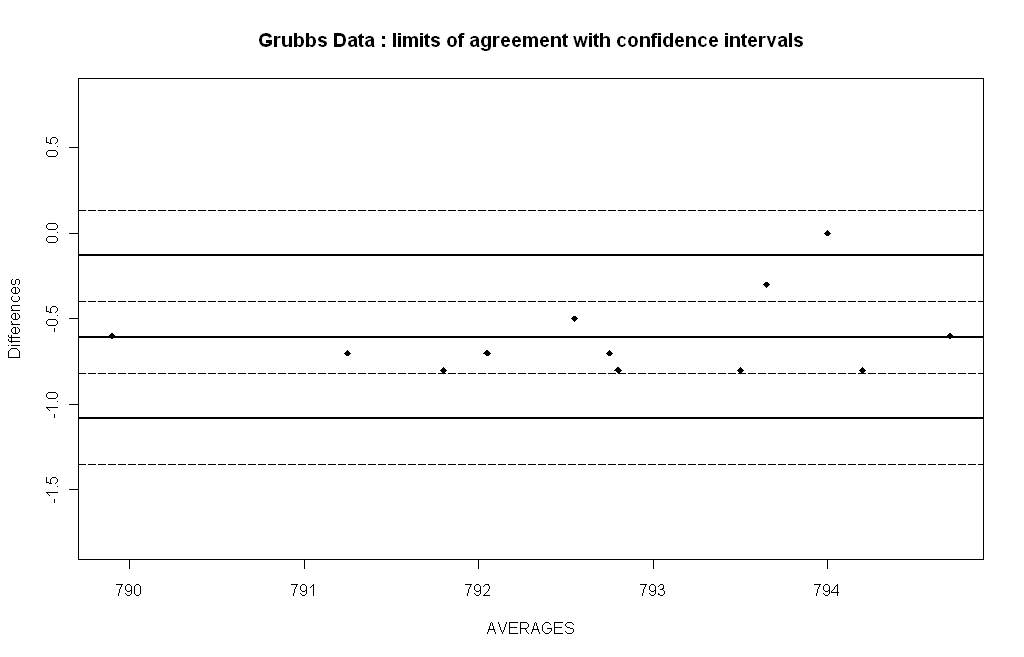
\includegraphics[width=125mm]{GrubbsLOAwCIs.jpeg}
%  \caption{Limits of agreement with confidence intervals}\label{LOAwCIs}
%\end{center}
%\end{figure}

%\newpage
%\section{Agreement Indices}
%\citet{Barnhart} provided an overview of several agreement
%indices, including the limits of agreement. Other approaches, such
%as mean squared deviation, the tolerance deviation index and
%coverage probability are also discussed.

\subsection{Alternative agreement indices}
As an alternative to limits of agreement, \citet{lin2002} proposes the use of
the mean square deviation is assessing agreement. The mean square
deviation is defined as the expectation of the squared differences
of two readings . The MSD is usually used for the case of two
measurement methods $X$ and $Y$ , each making one measurement for
the same subject, and is given by
\[
MSDxy = E[(x - y)^2]  = (\mu_{x} - \mu_{y})^2 + (\sigma_{x} -
\sigma_{y})^2 + 2\sigma_{x}\sigma_{y}(1-\rho_{xy}).
\]


\citet{Barnhart} advises the use of a predetermined upper limit
for the MSD value, $MSD_{ul}$, to define satisfactory agreement.
However, a satisfactory upper limit may not be properly
determinable, thus creating a drawback to this methodology.


\citet{Barnhart} proposes both the use of the square root of the
MSD or the expected absolute difference (EAD) as an alternative agreement indices. Both of these indices can be interpreted intuitively, being denominated in the same units of measurements as the original
measurements. Also they can be compare to the maximum acceptable
absolute difference between two methods of measurement $d_{0}$.
\[
EAD = E(|x - y|) = \frac{\sum |x_{i}- y_{i}|}{n}
\]

The EAD can be used to supplement the inter-method bias in an
initial comparison study, as the EAD is informative as a measure
of dispersion, is easy to calculate and requires no distributional
assumptions.

\citet{Barnhart} remarks that a comparison of EAD and MSD , using
simulation studies, would be interesting, while further adding
that `It will be of interest to investigate the benefits of these
possible new unscaled agreement indices'. For the Grubbs' `F vs C' and `F vs T' comparisons, the inter-method bias, difference variances, limits of agreement and EADs are shown
in Table 1.5. The corresponding Bland-Altman plots for `F vs C' and `F vs T' comparisons were depicted previously on Figure 1.3. While the inter-method bias for the `F vs T' comparison is smaller, the EAD penalizes the comparison for having a greater variance of differences. Hence the EAD values for both comparisons are much closer.
\begin{table}[ht]
\begin{center}
\begin{tabular}{|c|c|c|}
  \hline
 & F vs C & F vs T  \\
  \hline
Inter-method bias & -0.61 & 0.12 3 \\
Difference variances & 0.06 & 0.22  \\
Limits of agreement & (-1.08,	-0.13) & (-0.81,1.04) \\
  EAD & 0.61 & 0.35  \\
   \hline
\end{tabular}
\caption{Agreement indices for Grubbs' data comparisons.}
\end{center}
\end{table}

Further to  \citet{lin2000} and \citet{lin2002}, individual agreement between two measurement methods may be
assessed using the the coverage probability (CP) criteria or the total deviation index (TDI). If $d_{0}$ is predetermined as the maximum acceptable absolute difference between two methods of measurement, the probability that the absolute difference of two measures being less than $d_{0}$ can be computed. This is known as the coverage probability (CP).

\begin{equation}
CP = P(|x_{i} - y_{i}| \leq d_{0})
\end{equation}

If $\pi_{0}$ is set as the predetermined coverage probability, the
boundary under which the proportion of absolute differences is
$\pi_{0}$ may be determined. This boundary is known as the `total
deviation index' (TDI). Hence the TDI is the $100\pi_{0}$
percentile of the absolute difference of paired observations.

\section{Variations of the Bland-Altman Plot} Referring to the
assumption that bias and variability are constant across the range
of measurements, \citet{BA99} address the case where there is an
increase in variability as the magnitude increases. They remark
that it is possible to ignore the issue altogether, but the limits
of agreement would wider apart than necessary when just lower
magnitude measurements are considered. Conversely the limits would
be too narrow should only higher magnitude measurements be used.
To address the issue, they propose the logarithmic transformation
of the data. The plot is then formulated as the difference of
paired log values against their mean. Bland and Altman acknowledge
that this is not easy to interpret, and may not be suitable in
all cases.

\citet{BA99} offers two variations of the Bland-Altman plot that
are intended to overcome potential problems that the conventional
plot would inappropriate for. The first variation is a plot of
case-wise differences as percentage of averages, and is
appropriate when there is an increase in variability of the
differences as the magnitude increases. The second variation is a
plot of case-wise ratios as percentage of averages. This will
remove the need for $log$ transformation. This approach is useful
when there is an increase in variability of the differences as the
magnitude of the measurement increases. \citet{Eksborg} proposed
such a ratio plot, independently of Bland and Altman.
\citet{Dewitte} commented on the reception of this article by
saying `Strange to say,this report has been overlooked'.

\subsection{Replicate Measurements}

Thus far, the formulation for comparison of two measurement
methods is one where one measurement by each method is taken on
each subject. Should there be two or more measurements by each
methods, these measurement are known as `replicate measurements'.
\citet{BXC2008} recommends the use of replicate measurements, but
acknowledges the additional computational complexity.

\citet*{BA86} address this problem by offering two different
approaches. The premise of the first approach is that replicate
measurements can be treated as independent measurements. The
second approach is based upon using the mean of the each group of
replicates as a representative value of that group. Using either
of these approaches will allow an analyst to estimate the inter
method bias.

%\subsubsection{Mean of Replicates Limits of Agreement}

However, because of the removal of the effects of the replicate
measurements error, this would cause the estimation of the
standard deviation of the differences to be unduly small.
\citet*{BA86} propose a correction for this.

\citet{BXC2008} takes issue with the limits of agreement based on
mean values of replicate measurements, in that they can only be interpreted as prediction
limits for difference between means of repeated measurements by
both methods, as opposed to the difference of all measurements.
Incorrect conclusions would be caused by such a misinterpretation.
\citet{BXC2008} demonstrates how the limits of agreement
calculated using the mean of replicates are `much too narrow as
prediction limits for differences between future single
measurements'. This paper also comments that, while treating the
replicate measurements as independent will cause a downward bias
on the limits of agreement calculation, this method is preferable
to the `mean of replicates' approach.



%%%%%%%%%%%%%%%%%%%%%%%%%%%%%%%%%%%%%%%%%%%%%%%%%%%%%%%%%%%%%%%%%%%%%%%%%%%%%%%%%%%%%%%
\newpage
\section{Formal Models and Tests}
The Bland-Altman plot is a simple tool for inspection of data, and
\citet{Kinsella} comments on the lack of formal testing offered by
that methodology. \citet{Kinsella} formulates a model for
single measurement observations for a method comparison study as a
linear mixed effects model, i.e. model that additively combine
fixed effects and random effects.
\[
Y_{ij} =\quad \mu + \beta_{j} + u_{i} + \epsilon_{ij} \qquad i = 1,\dots,n
\qquad j=1,2\]

The true value of the measurement is represented by $\mu$ while the fixed effect due to method $j$ is $\beta_{j}$.
For simplicity these terms can be combined into single terms; $\mu_{1} = \mu+ \beta_{1}$ and $\mu_{2} = \mu + \beta_{2}$. The inter-method bias is the difference of the two fixed effect terms, $\beta_{1}-\beta_{2}$. Each of the $i$ individuals are assumed to give rise to random error, represented by $u_{i}$. This random effects terms is assumed to have mean zero and be normally distributed with variance $\sigma^2$. There is assumed to be an attendant error for each measurement on each individual, denoted $\epsilon_{ij}$. This is also assumed to have mean zero. The variance of measurement error for both methods are not assumed to be identical for both methods variance,  hence it is denoted $\sigma^2_{j}$. The set of observations ($x_{i},y_{i}$) by methods $X$ and $Y$ are assumed to follow the bivariate normal distribution with expected values $E(x_{i})= \mu_{i}$ and $E(x_{i})= \mu_{i}$ respectively. The variance covariance of the observations $\boldsymbol{\Sigma}$ is given by

\[
\boldsymbol{\Sigma} = \left[
                        \begin{array}{cc}
                          \sigma^{2} + \sigma^{2}_{1} & \sigma^{2} \\
                          \sigma^{2} & \sigma^{2} + \sigma^{2}_{2} \\
                        \end{array}
                      \right]
\]

The inter-method bias is the difference of the two fixed effect terms, $\beta_{1}-\beta_{2}$.

\citet{Kinsella} demonstrates the estimation of the variance terms and relative precisions relevant to a method comparison study, with attendant confidence intervals for both. The measurement model introduced by \citet{Grubbs48,Grubbs73} provides a formal procedure for estimate the variances $\sigma^2$,$\sigma^2_{1}$ and $\sigma^2_{2}$ devices. \citet{Grubbs48} offers estimates, commonly known as Grubbs estimators, for the various variance components. These estimates are maximum likelihood estimates, a statistical concept that shall be revisited in due course.
\begin{eqnarray*}
\hat{\sigma^{2}} = \sum{\frac{(x_{i}-\bar{x})(y_{i}-\bar{y})}{n-1}} = Sxy\\
\hat{\sigma^{2}_{1}} = \sum{\frac{(x_{i}-\bar{x})^{2}}{n-1}} =S^{2}x - Sxy  \\
\hat{\sigma^{2}_{2}} =
\sum{\frac{(y_{i}-\bar{y})^{2}}{n-1}} = S^{2}y - Sxy
\end{eqnarray*}

% The standard error of these variance estimates are:
% \begin{eqnarray}
% \mbox{var}(\sigma^{2}_{1}) = \frac{2\sigma^{4}_{1}}{n-1} +
% \frac{\sigma^2_{S}\sigma^2_{1}+\sigma^2_{S}\sigma^2_{2}+\sigma^2_{1}\sigma^2_{2}
% }{n-1}\\
% \mbox{var}(\sigma^{2}_{2}) =\quad \frac{2\sigma^{4}_{2}}{n-1} +
% \frac{\sigma^2_{S}\sigma^2_{1}+\sigma^2_{S}\sigma^2_{2}+\sigma^2_{1}\sigma^2_{2}
% }{n-1}\nonumber
% \end{eqnarray}

\citet{Thompson} defines $\Delta_{j}$ to be a measure of the
relative precision of the measurement methods, with $\Delta_{j}=
\sigma^2/\sigma^2_{j}$. Thompson also demonstrates how to make statistical inferences about $\Delta_{j}$.
Based on the following identities,
\begin{eqnarray*}
C_{x}&=&(n-1)S^2_{x},\nonumber\\
C_{xy}&=&(n-1)S_{xy},\nonumber\\
C_{y}&=&(n-1)S^2_{y},\nonumber\\
|A| &=& C_{x}\times C_{y} - (C_{xy})^2,\nonumber
\end{eqnarray*}
\noindent the confidence interval limits of $\Delta_{1}$ are

\begin{eqnarray}
\Delta_{1} > \frac{C_{xy}-
t(\frac{|A|}{n-2}))^{\frac{1}{2}}}{C_{x}-C_{xy}+
t(\frac{|A|}{n-2}))^{\frac{1}{2}}} \\
\Delta_{1} > \frac{C_{xy}+
t(\frac{|A|}{n-2}))^{\frac{1}{2}}}{C_{x}-C_{xy}-
t(\frac{|A|}{n-1}))^{\frac{1}{2}}} \nonumber
\end{eqnarray}
\\ The value $t$ is the $100(1-\alpha/2)\%$ upper quantile of
Student's $t$ distribution with $n-2$ degrees of freedom
\citep{Kinsella}. The confidence limits for $\Delta_{2}$ are found by substituting $C_{y}$ for $C_{x}$ in (1.3).
Negative lower limits are replaced by the value $0$.

%For the interval estimates for the variance components,
%\citet{Thompson} presents three relations that hold simultaneously
%with probability $1-2\alpha$ where $2\alpha=0.01$ or $0.05$.

%\begin{eqnarray*}
%|\sigma^2-C_{xy}K| &\leqslant& M(C_{x}C_{y})^{\frac{1}{2}}\\
%|\sigma^2_{1}-(C_{x}-C_{xy})K|&\leqslant M(C_{x}(C_{x}+C_{y}-2C_{xy}))^{\frac{1}{2}}\nonumber\\
%|\sigma^2_{2}-(C_{y}-C_{xy})K|&\leqslant
%M(C_{y}(C_{x}+C_{y}-2C_{xy}))^{\frac{1}{2}}\nonumber
%\end{eqnarray*}

%\citet{Thompson} contains tables for $K$ and $M$.

The case-wise differences and means are calculated as $d_{i} =
x_{i}-y_{i}$ and $a_{i} = (x_{i}+y_{i})/2$  respectively. Both
$d_{i}$ and $a_{i}$ are assumed to follow a bivariate normal
distribution with $E(d_{i})= \mu_{d} = \mu_{1} - \mu_{2}$ and
$E(a_{i})= \mu_{a} = (\mu_{1} + \mu_{2})/2$. The variance matrix
$\Sigma_{(a,d)}$ is

\begin{eqnarray}
\Sigma_{(a,d)}= \left[\begin{matrix}
\sigma^{2}_{1}+\sigma^{2}_{2}&\frac{1}{2}(\sigma^{2}_{1}-\sigma^{2}_{2})\\
\frac{1}{2}(\sigma^{2}_{1}-\sigma^{2}_{2})&\sigma^{2}+
\frac{1}{4}(\sigma^{2}_{1}+\sigma^{2}_{2})
\end{matrix} \right].
\end{eqnarray}



\subsection{Morgan Pitman Testing}
An early contribution to formal testing in method comparison was
made by both \citet{morgan} and \citet{pitman}, in separate
contributions. The basis of this approach is that if the
distribution of the original measurements is bivariate normal.
Morgan and Pitman noted that the correlation coefficient depends
upon the difference $\sigma^{2}_{1}- \sigma^{2}_{2}$, being zero
if and only if $\sigma^{2}_{1}=\sigma^{2}_{2}$.

The classical Pitman-Morgan test is a hypothesis test for equality
of the variance of two data sets; $\sigma^{2}_{1} =
\sigma^{2}_{2}$, based on the correlation value $\rho_{a,d}$ ,and
is evaluated as follows;

\begin{equation}
\rho(a,d)=\quad\frac{\sigma^{2}_{1}-\sigma^{2}_{2}}{\sqrt{(\sigma^{2}_{1}+\sigma^{2}_{2})(4\sigma^{2}_{S}+\sigma^{2}_{1}+\sigma^{2}_{2})}}
\end{equation}

The correlation constant takes the value zero if, and only if, the two variances are equal. Therefore a test of the hypothesis $H: \sigma^{2}_{1}=\sigma^{2}_{2}$ is equivalent to a test of the hypothesis $H: \rho(D,A) = 0$. The corresponds to the well-known
$t$ test for a correlation coefficient with $n-2$ degrees of freedom. \citet{Bartko} describes the Morgan-Pitman test as identical to
the test of the slope equal to zero in the regression of $Y_{i1}$ on $Y_{12}$, a result that can be derived using
straightforward algebra.


\subsection{Paired sample \emph{t} test}

\citet{Bartko} discusses the use of the well known paired sample
$t$ test to test for inter-method bias; $H: \mu_{d}=0$. The test
statistic is distributed a $t$ random variable with $n-1$ degrees
of freedom and is calculated as follows,

\begin{equation}
t^{*} = \frac{\bar{d}}{ \frac{s_{d}}{\sqrt{n}}}
\end{equation}

where $\bar{d}$ and $s_{d}$ is the average of the differences of
the $n$ observations. Only if the two methods show comparable
precision then the paired sample student t-test is appropriate for
assessing the magnitude of the bias.
\begin{eqnarray}
t^{*} = \frac{\bar{d}}{s_{d}/\sqrt{n}}
\end{eqnarray}

\subsection{Bland-Altman correlation test}

The approach proposed by \citet{BA83} is a formal test on the
Pearson correlation coefficient of case-wise differences and means
($\rho_{AD}$). According to the authors, this test is equivalent
to the `Pitman Morgan Test'. For the Grubbs data, the correlation
coefficient estimate ($r_{AD}$) is 0.2625, with a 95\% confidence
interval of (-0.366, 0.726) estimated by Fishers `$r$ to $z$'
transformation \citep*{Cohen}. The null hypothesis ($\rho_{AD}$ =0)
fail to be rejected. Consequently the null hypothesis of equal
variances of each method would also fail to be rejected. There has
no been no further mention of this particular test in
\citet{BA86}, although \citet{BA99} refers to Spearman's rank
correlation coefficient. \citet{BA99} comments `we do not see a
place for methods of analysis based on hypothesis testing'.
\citet{BA99} also states that consider structural equation models
to be inappropriate.

\subsection{Identifiability}
\citet{DunnSEME} highlights an important issue regarding using
models such as these, the identifiability problem. This comes as a
result of there being too many parameters to be estimated.
Therefore assumptions about some parameters, or estimators used,
must be made so that others can be estimated. For example in literature the variance
ratio $\lambda=\frac{\sigma^{2}_{1}}{\sigma^{2}_{2}}$
must often be assumed to be equal to $1$ \citep{linnet98}.\citet{DunnSEME} considers methodologies based on two methods with single measurements on each subject as inadequate for a serious
study on the measurement characteristics of the methods. This is
because there would not be enough data to allow for a meaningful
analysis. There is, however, a contrary argument that in many
practical settings it is very difficult to get replicate
observations when the measurement method requires invasive medical
procedure.

%%%%%%%%%%%%%%%%%%%%%%%%%%%%%%%%%%%%%%%%%%%%%%%%%%%%%%%%%%%%%%%%%%%%%%%%%%%%%%%Bartko's BB
\citet{BB89} offers a formal simultaneous hypothesis test for the
mean and variance of two paired data sets. Using simple linear
regression of the differences of each pair against the sums, a
line is fitted to the model, with estimates for intercept and
slope ($\hat{\beta}_{0}$ and $\hat{\beta}_{1}$). The null
hypothesis of this test is that the mean ($\mu$) and variance
($\sigma^{2}$) of both data sets are equal if the slope and
intercept estimates are equal to zero(i.e $\sigma^{2}_{1} =
\sigma^{2}_{2}$ and $\mu_{1}=\mu_{2}$ if and only if $\beta_{0}=
\beta_{1}=0$ )

A test statistic is then calculated from the regression analysis
of variance values \citep{BB89} and is distributed as `$F$' random
variable. The degrees of freedom are $\nu_{1}=2$ and $\nu_{1}=n-2$
(where $n$ is the number of pairs). The critical value is chosen
for $\alpha\%$ significance with those same degrees of freedom.
\citet{Bartko} amends this methodology for use in method
comparison studies, using the averages of the pairs, as opposed to
the sums, and their differences. This approach can facilitate
simultaneous usage of test with the Bland-Altman methodology.
Bartko's test statistic take the form:
\[ F.test = \frac{(\Sigma d^{2})-SSReg}{2MSReg}
\]
% latex table generated in R 2.6.0 by xtable 1.5-5 package
% Mon Aug 31 15:53:51 2009
\begin{table}[ht]
\begin{center}
\begin{tabular}{lrrrrr}
  \hline
 & Df & Sum Sq & Mean Sq & F value & Pr($>$F) \\
  \hline
Averages & 1 & 0.04 & 0.04 & 0.74 & 0.4097 \\
  Residuals & 10 & 0.60 & 0.06 &  &  \\
   \hline
\end{tabular}
\caption{Regression ANOVA of case-wise differences and averages
for Grubbs Data}
\end{center}
\end{table}
%(calculate using R code $qf(0.95,2,10)$).

For the Grubbs data, $\Sigma d^{2}=5.09 $, $SSReg = 0.60$ and
$MSreg=0.06$ Therefore the test statistic is $37.42$, with a
critical value of $4.10$. Hence the means and variance of the
Fotobalk and Counter chronometers are assumed to be simultaneously
equal.

Importantly, this methodology determines whether there is both
inter-method bias and precision present, or alternatively if there
is neither present. It has previously been demonstrated that there
is a inter-method bias present, but as this procedure does not
allow for separate testing, no conclusion can be drawn on the
comparative precision of both methods.



%This application of the
%Grubbs method presumes the existence of this condition, and necessitates
%replication of observations by means external to and independent of the first
%means. The Grubbs estimators method is based on the laws of propagation of
%error. By making three independent simultaneous measurements on the same
%physical material, it is possible by appropriate mathematical manipulation of
%the sums and differences of the associated variances to obtain a valid
%estimate of the precision of the primary means. Application of the Grubbs
%estimators procedure to estimation of the precision of an apparatus uses
%the results of a physical test conducted in such a way as to obtain a series
%of sets of three independent observations.


\section{Regression Methods}
Conventional regression models are estimated using the ordinary
least squares (OLS) technique, and are referred to as `Model I
regression' \citep{CornCoch,ludbrook97}. A key feature of Model I
models is that the independent variable is assumed to be measured
without error. As often pointed out in several papers
\citep{BA83,ludbrook97}, this assumption invalidates simple linear
regression for use in method comparison studies, as both methods
must be assumed to be measured with error.

The use of regression models that assumes the presence of error in
both variables $X$ and $Y$ have been proposed for use instead
\citep{CornCoch,ludbrook97}. These methodologies are collectively
known as `Model II regression'. They differ in the method used to
estimate the parameters of the regression.

Regression estimates depend on formulation of the model. A
formulation with one method considered as the $X$ variable will
yield different estimates for a formulation where it is the $Y$
variable. With Model I regression, the models fitted in both cases
will entirely different and inconsistent. However with Model II
regression, they will be consistent and complementary.

Regression approaches are useful for a making a detailed examination of the biases across the range of measurements, allowing bias to be decomposed into fixed bias and proportional bias.
Fixed bias describes the case where one method gives values that are consistently different
to the other across the whole range. Proportional
bias describes the difference in measurements getting progressively greater, or smaller, across the range of measurements. A measurement method may have either an attendant fixed bias or proportional bias, or both. \citep{ludbrook}. Determination of these biases shall be discussed in due course.


\subsection{Deming Regression}

As stated previously, the fundamental flaw of simple linear regression is that it allows for measurement error in one variable only. This causes a downward biased slope estimate.

Deming regression is a regression fitting approach that assumes error in both variables. Deming regression is recommended by \citet*{CornCoch} as the
preferred Model II regression for use in method comparison
studies.
The sum of squared distances from measured sets of values to the regression line is minimized at an angles specified by the ratio $\lambda$ of the residual variance of both variables. I
When $\lambda$ is one, the angle is 45 degrees. In ordinary linear regression, the distances are minimized in the vertical directions \citep{linnet99}.
In cases involving only single measurements by each method, $\lambda$ may be unknown and is therefore assumes a value of one. While this will bias the estimates, it is less biased than ordinary linear regression.

The Bland Altman Plot is
uninformative about the comparative influence of proportional bias
and fixed bias. Model II approaches, such as Deming regression,  can provide independent tests for
both types of bias.

For a given $\lambda$, \citet{Kummel} derived the following
estimate that would later be used for the Deming regression slope
parameter. The intercept estimate $\alpha$
is simply estimated in the same way as in conventional linear
regression, by using the identity $\bar{Y}-\hat{\beta}\bar{X}$;
\begin{equation}
\hat{\beta} =\quad \frac{S_{yy} - \lambda S_{xx}+[(S_{yy} -
\lambda S_{xx})^{2}+ 4\lambda S^{2}_{xy}]^{1/2}}{2S_{xy}}
\end{equation},
with $\lambda$ as the variance ratio. As stated previously $\lambda$ is often unknown, and therefore must be assumed to equal one. \citet{CarollRupert} states that Deming
regression is acceptable only when the precision ratio ($\lambda$,in their paper as $\eta$) is correctly specified, but in practice this is often not the case, with the $\lambda$ being underestimated. Several candidate models, with varying variance ratios may be fitted, and estimates of the slope and intercept are produced. However no model selection information is available to determine the best fitting model.

As with conventional regression methodologies, Deming regression
calculates an estimate for both the slope and intercept for the
fitted line, and standard errors thereof. Therefore there is
sufficient information to carry out hypothesis tests on both
estimates, that are informative about presence of fixed and
proportional bias.

A $95\%$ confidence interval for the intercept estimate can be
used to test the intercept, and hence fixed bias, is equal to
zero. This hypothesis is accepted if the confidence interval for
the estimate contains the value $0$ in its range. Should this be,
it can be concluded that fixed bias is not present. Conversely, if
the hypothesis is rejected, then it is concluded that the
intercept is non zero, and that fixed bias is present.

Testing for proportional bias is a very similar procedure. The
$95\%$ confidence interval for the slope estimate can be used to
test the hypothesis that the slope is equal to $1$. This
hypothesis is accepted if the confidence interval for the estimate
contains the value $1$ in its range. If the hypothesis is
rejected, then it is concluded that the slope is significant
different from $1$ and that a proportional bias exists.

For convenience, a new data set shall be introduced to demonstrate
Deming regression. Measurements of transmitral volumetric flow
(MF) by doppler echocardiography, and left ventricular stroke
volume (SV) by cross sectional echocardiography in 21 patients
with aortic valve disease are tabulated in \citet{zhang}. This
data set features in the discussion of method comparison studies
in \citet[p.398]{AltmanBook} .


% latex table generated in R 2.6.0 by xtable 1.5-5 package
% Tue Sep 01 13:31:17 2009
\begin{table}[h!]
\begin{center}
\begin{tabular}{|c|c|c||c|c|c||c|c|c|}
  \hline
 Patient & MF  & SV  & Patient & MF  & SV  & Patient & MF  & SV \\
 &($cm^{3}$)&  ($cm^{3}$) & &($cm^{3}$)&  ($cm^{3}$) & &($cm^{3}$)&  ($cm^{3}$)
 \\
  \hline
1 & 47 & 43 &  8 & 75 & 72 &  15 & 90 & 82 \\
  2 & 66 & 70 & 9 & 79 & 92 &  16 & 100 & 100 \\
  3 & 68 & 72 & 10 & 81 & 76 & 17 & 104 & 94 \\
  4 & 69 & 81 & 11 & 85 & 85 &  18 & 105 & 98 \\
  5 & 70 & 60 & 12 & 87 & 82 & 19 & 112 & 108 \\
  6 & 70 & 67 & 13 & 87 & 90 & 20 & 120 & 131 \\
  7 & 73 & 72 & 14 & 87 & 96 &  21 & 132 & 131 \\

   \hline
\end{tabular}
\caption{Transmitral volumetric flow(MF) and left ventricular
stroke volume (SV) in 21 patients. (Zhang et al 1986)}
\end{center}
\end{table}

\begin{figure}[h!]
  % Requires \usepackage{graphicx}
  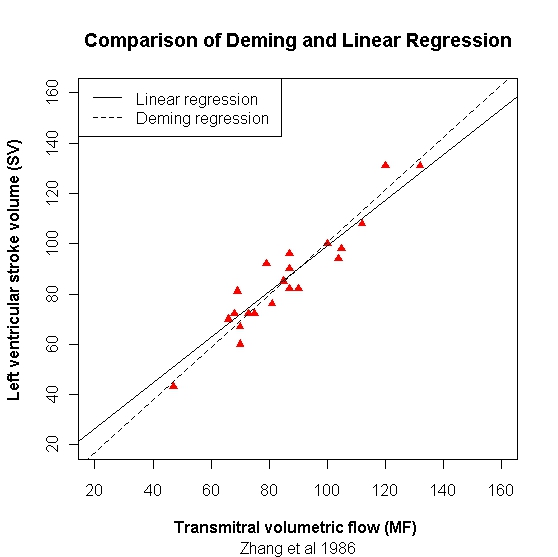
\includegraphics[width=130mm]{ZhangDeming.jpeg}
  \caption{Deming Regression For Zhang's Data}\label{ZhangDeming}
\end{figure}


\citet{CarollRupert} states that Deming's
regression is acceptable only when the precision ratio ($\lambda$,
in their paper as $\eta$) is correctly specified, but in practice
this is often not the case, with the $\lambda$ being
underestimated.
\newpage
\section{Other Types of Studies}
\citet{lewis} categorize method comparison studies into three
different types.  The key difference between the first two is
whether or not a `gold standard' method is used. In situations
where one instrument or method is known to be `accurate and
precise', it is considered as the`gold standard' \citep{lewis}. A
method that is not considered to be a gold standard is referred to
as an `approximate method'. In calibration studies they are
referred to a criterion methods and test methods respectively.


\textbf{1. Calibration problems}. The purpose is to establish a
relationship between methods, one of which is an approximate
method, the other a gold standard. The results of the approximate
method can be mapped to a known probability distribution of the
results of the gold standard \citep{lewis}. (In such studies, the
gold standard method and corresponding approximate method are
generally referred to a criterion method and test method
respectively.) \citet*{BA83} make clear that their methodology is
not intended for calibration problems.

\bigskip \textbf{2. Comparison problems}. When two approximate
methods, that use the same units of measurement, are to be
compared. This is the case which the Bland-Altman methodology is
specfically intended for, and therefore it is the most relevant of
the three.

\bigskip \textbf{3. Conversion problems}. When two approximate
methods, that use different units of measurement, are to be
compared. This situation would arise when the measurement methods
use 'different proxies', i.e different mechanisms of measurement.
\citet{lewis} deals specifically with this issue. In the context
of this study, it is the least relevant of the three.

\citet[p.47]{DunnSEME} cautions that`gold standards' should not be
assumed to be error free. `It is of necessity a subjective
decision when we come to decide that a particular method or
instrument can be treated as if it was a gold standard'. The
clinician gold standard , the sphygmomanometer, is used as an
example thereof.  The sphygmomanometer `leaves considerable room
for improvement' \citep{DunnSEME}. \citet{pizzi} similarly
addresses the issue of glod standards, `well-established gold
standard may itself be imprecise or even unreliable'.


The NIST F1 Caesium fountain atomic clock is considered to be the
gold standard when measuring time, and is the primary time and
frequency standard for the United States. The NIST F1 is accurate
to within one second per 60 million years \citep{NIST}.

Measurements of the interior of the human body are, by definition,
invasive medical procedures. The design of method must balance the
need for accuracy of measurement with the well-being of the
patient. This will inevitably lead to the measurement error as
described by \citet{DunnSEME}. The magnetic resonance angiogram,
used to measure internal anatomy,  is considered to the gold
standard for measuring aortic dissection. Medical test based upon
the angiogram is reported to have a false positive reporting rate
of 5\% and a false negative reporting rate of 8\%. This is
reported as sensitivity of 95\% and a specificity of 92\%
\citep{ACR}.

In literature they are, perhaps more accurately, referred to as
`fuzzy gold standards' \citep{phelps}. Consequently when one of the methods is
essentially a fuzzy gold standard, as opposed to a `true' gold
standard, the comparison of the criterion and test methods should
be consider in the context of a comparison study, as well as of a
calibration study.

\newpage
\section{Outline of Thesis}
Thus the study of method comparison is introduced. The intention of this thesis is to progress the
study of method comparison studies, using a statistical method known as Linear mixed effects models.
Chapter two shall describe linear mixed effects models, and how the use of the linear mixed
effects models have so far extended to method comparison studies. Implementations of important existing work shall be presented, using the \texttt{R} programming language.

Model diagnostics are an integral component of a complete statistical analysis.
In chapter three model diagnostics shall be described in depth, with particular
emphasis on linear mixed effects models, further to chapter two.

For the fourth chapter, important linear mixed effects model diagnostic methods shall be extended to method comparison studies, and proposed methods shall be demonstrated on data sets that have become well known in literature on method comparison. The purpose is to both calibrate these methods and to demonstrate applications for them.
The last chapter shall focus on robust measures of important parameters such as agreement.

%%%%%%%%%%%%%%%%%%%%%%%%%%%%%%%%%%%%%%%%%%%%%%%%%%%%%%%%%%%%%%%%%%%%%%%%%%%%%%%%%%%%%%%%%%%%%%%%%%%%%%%%%%%%%%%%%%%%%
%%%%%%%%%%%%%%%%%%%%%%%%%%%%%%%%%%%%%%%%%%%%%%%%%%%%%%%%%%%%%%%%%%%%%%%%%%%%%%%%%%%%%%%%%%%%%%%%%%%%%%%%%%%%%%%%%%%%%



\end{document}
